
\documentclass{exam}

\usepackage{fullpage}
\usepackage{enumerate}
\usepackage{siunitx} 
\usepackage{graphicx}
\usepackage[fleqn]{amsmath}
\usepackage{cancel}
\usepackage{polynom}
\usepackage{float}
\usepackage{mdwlist}
\usepackage{booktabs}
\usepackage{cancel}
\usepackage{polynom}
\usepackage{caption}

\newcommand{\degree}{\ensuremath{^\circ}} 
\everymath{\displaystyle}

% \begin{figure}[H]
%   \centering
%   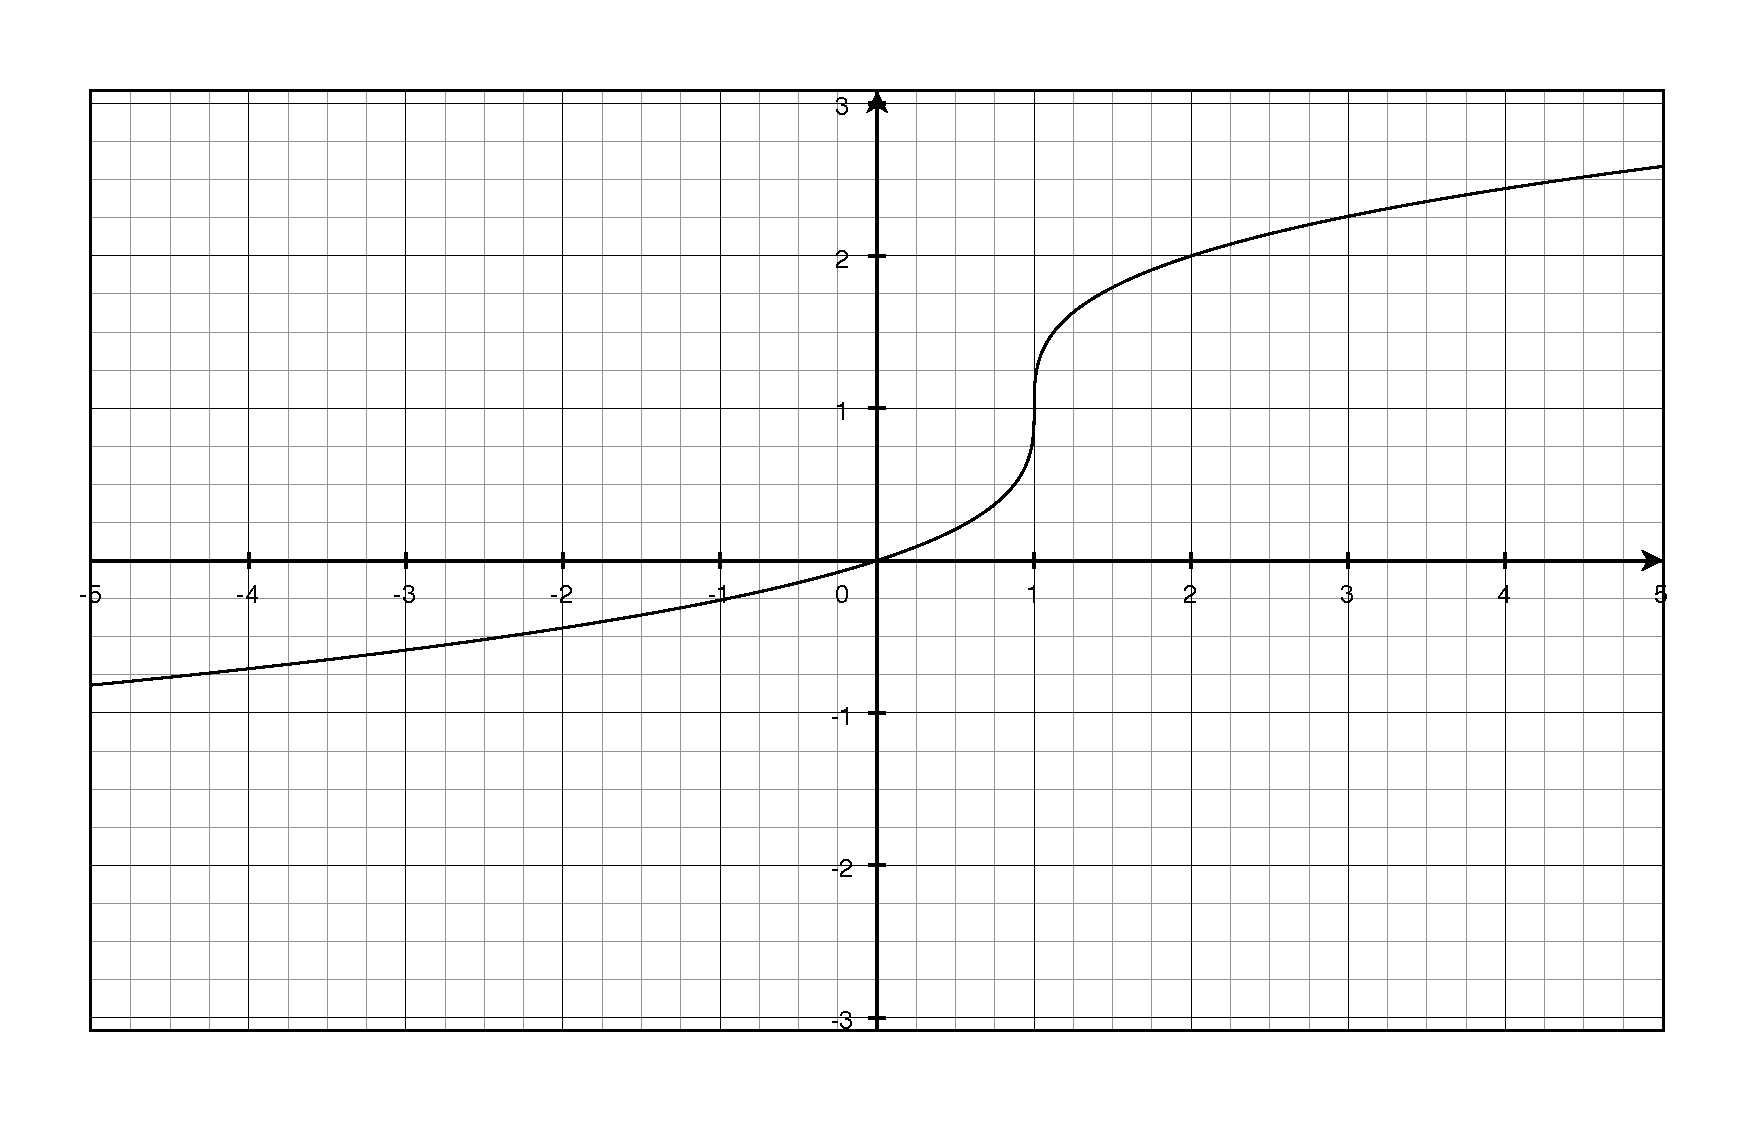
\includegraphics[scale=.3]{question7.eps}
%   \caption*{Question 7}
% \end{figure}

% \begin{tabular}{cc}
% \toprule
% period & amplitude \\
% \midrule
%   $\pi$ & $2$ \\
% \bottomrule
% \end{tabular}

% \textwidth 6.5 in

\printanswers

\ifprintanswers 
\usepackage{2in1, lscape} 
\fi

\title{Math 263a \\ Homework Three}
\date{February 1, 2012}

\begin{document}

  \maketitle

  \section{Homework}

  \begin{itemize*}
    \item Read Section 2.4-2.5
    \item pp 70-71: 5-8, 13-16, 27-28, 30
    \item pp 78-79: 2, 7-12
  \end{itemize*}

  \section{Extra Credit}
  \begin{itemize*}
  \item pp 70-71: 34 and 36
  % \item pp 78: 27
  \end{itemize*}

  \ifprintanswers

  \begin{description}
    \item[34]
    \begin{align*}
      \lim_{x \to 0} \frac{\sqrt{x+2} - \sqrt{2}}{x} 
        &= \lim_{x \to 0} \left( \frac{\sqrt{x+2} - \sqrt{2}}{x} \right) \left( \frac{\sqrt{x+2} + \sqrt{2}}{\sqrt{x+2} + \sqrt{2}} \right) \\
        &= \lim_{x \to 0} \frac{x+2 - 2}{x(\sqrt{x+2} + \sqrt{2})}  \\
        &= \lim_{x \to 0} \frac{x}{x(\sqrt{x+2} + \sqrt{2})} \\
        &= \lim_{x \to 0} \frac{1}{\sqrt{x+2} + \sqrt{2}} \\
        &= \frac{1}{2 \sqrt{2}} \\
        &= \frac{\sqrt{2}}{4} \\
    \end{align*}
  \end{description}

  \section{Section 2.4}
  \begin{description}
    \item[5]
    \[
      \lim_{t \to -1} \frac{1-2t}{\sqrt{3t + 21}} = \frac{1 + 2}{\sqrt{-3 + 21}} = \frac{3}{\sqrt{18}} = \frac{\sqrt{2}}{2}
    \]

    \item[6]
    \[
      \lim_{t \to -1} \frac{\sqrt{1-2t}}{(3t + 2)^3} = \frac{\sqrt{3}}{(-1)^3} = - \sqrt{3}
    \]

    \item[7]
    \begin{align*}
      \lim_{x \to 2} \frac{x^2 - 4}{x-2} &=   \lim_{x \to 2} \frac{(x+2)(x-2)}{x-2} \\
      &= \lim_{x \to 2} x+2 \\
      &= 4 \\
    \end{align*}

    \item[8]
    \begin{align*}
      \lim_{t \to -7} \frac{t^2 + 4t - 21}{t+7} &= \lim_{t \to -7} \frac{(t-3)(t+7)}{t+7} \\
      &= \lim_{t \to -7} t-3 \\
      &= -10 \\
    \end{align*}

    \item[13]
    \begin{align*}
      \lim_{t \to 2} \frac{\sqrt{(t+4)(t-2)^4}}{(3t-6)^2} &= \lim_{t \to 2} \frac{(t-2)^2\sqrt{t+4}}{3^2(t-2)^2} \\
      &= \lim_{t \to 2} \frac{\sqrt{t+4}}{9} \\
      &= \frac{\sqrt{6}}{9} \\
    \end{align*}

    \item[14]
    \begin{align*}
      \lim_{t \to 7} \frac{\sqrt{(t-7)^3}}{t-7} &= \lim_{t \to 7} \frac{(t-7)\sqrt{t-7}}{t-7} \\
      &= \lim_{t \to 7} \sqrt{t-7} \\
      &= 0 \\
    \end{align*}

    \item[15]
    \begin{align*}
       \lim_{x \to 3} \frac{x^4 - 18x^2 + 81}{(x-3)^2} &= \lim_{x \to 3} \frac{(x^2 - 9)^2}{(x-3)^2} \\
       &= \lim_{x \to 3} \frac{(x + 3)^2(x-3)^2}{(x-3)^2} \\
       &= \lim_{x \to 3} (x + 3)^2 \\
       &= 36 \\
    \end{align*}

    \item[16]
    \begin{align*}
       \lim_{u \to 1} \frac{(3u + 4)(2u-2)^3}{(u-1)^2} &=  \lim_{u \to 1} \frac{2^3(3u + 4)(u-1)^3}{(u-1)^2} \\
       &= \lim_{u \to 1} 8 (3u + 4)(u-1) \\  
       &= 0 \\
    \end{align*}

    \item[27]
    \begin{enumerate}[(a)]

    \item $\lim_{x \to -3} f(x) = 2$
    \item $f(-3) = 1$
    \item $f(-1)$ is not defined
    \item $\lim_{x \to -1} f(x) = 2.5$

    \item $f(1) = 2$
    \item $\lim_{x \to 1} f(x)$ is not defined since it the limit is different depending on which direction you approach 1 from.

    \item $\lim_{x \to 1^-} f(x) = 2$ 
    \item $\lim_{x \to 1^+} f(x) = 1$ 

    \end{enumerate}

    \item[28]
    \begin{enumerate}[(a)]

    \item $\lim_{x \to -3} f(x)$ is not defined since the limit is different depending on which direction you approach $-3$ from.
    \item $f(-3) = 1$

    \item $f(-1) = 1$
    \item $\lim_{x \to -1} f(x) = 2$

    \item $f(1) = 1$
    \item $\lim_{x \to 1} f(x)$ is not defined since the function appears to oscillate between 0.75 and 1.25 when approaching 1
      from the positive side.

    \item $\lim_{x \to 1^-} f(x) = 1$ 
    \item $\lim_{x \to 1^+} f(x)$ is not defined

    \end{enumerate}

    \item[30]
    \begin{figure}[H]
      \centering
      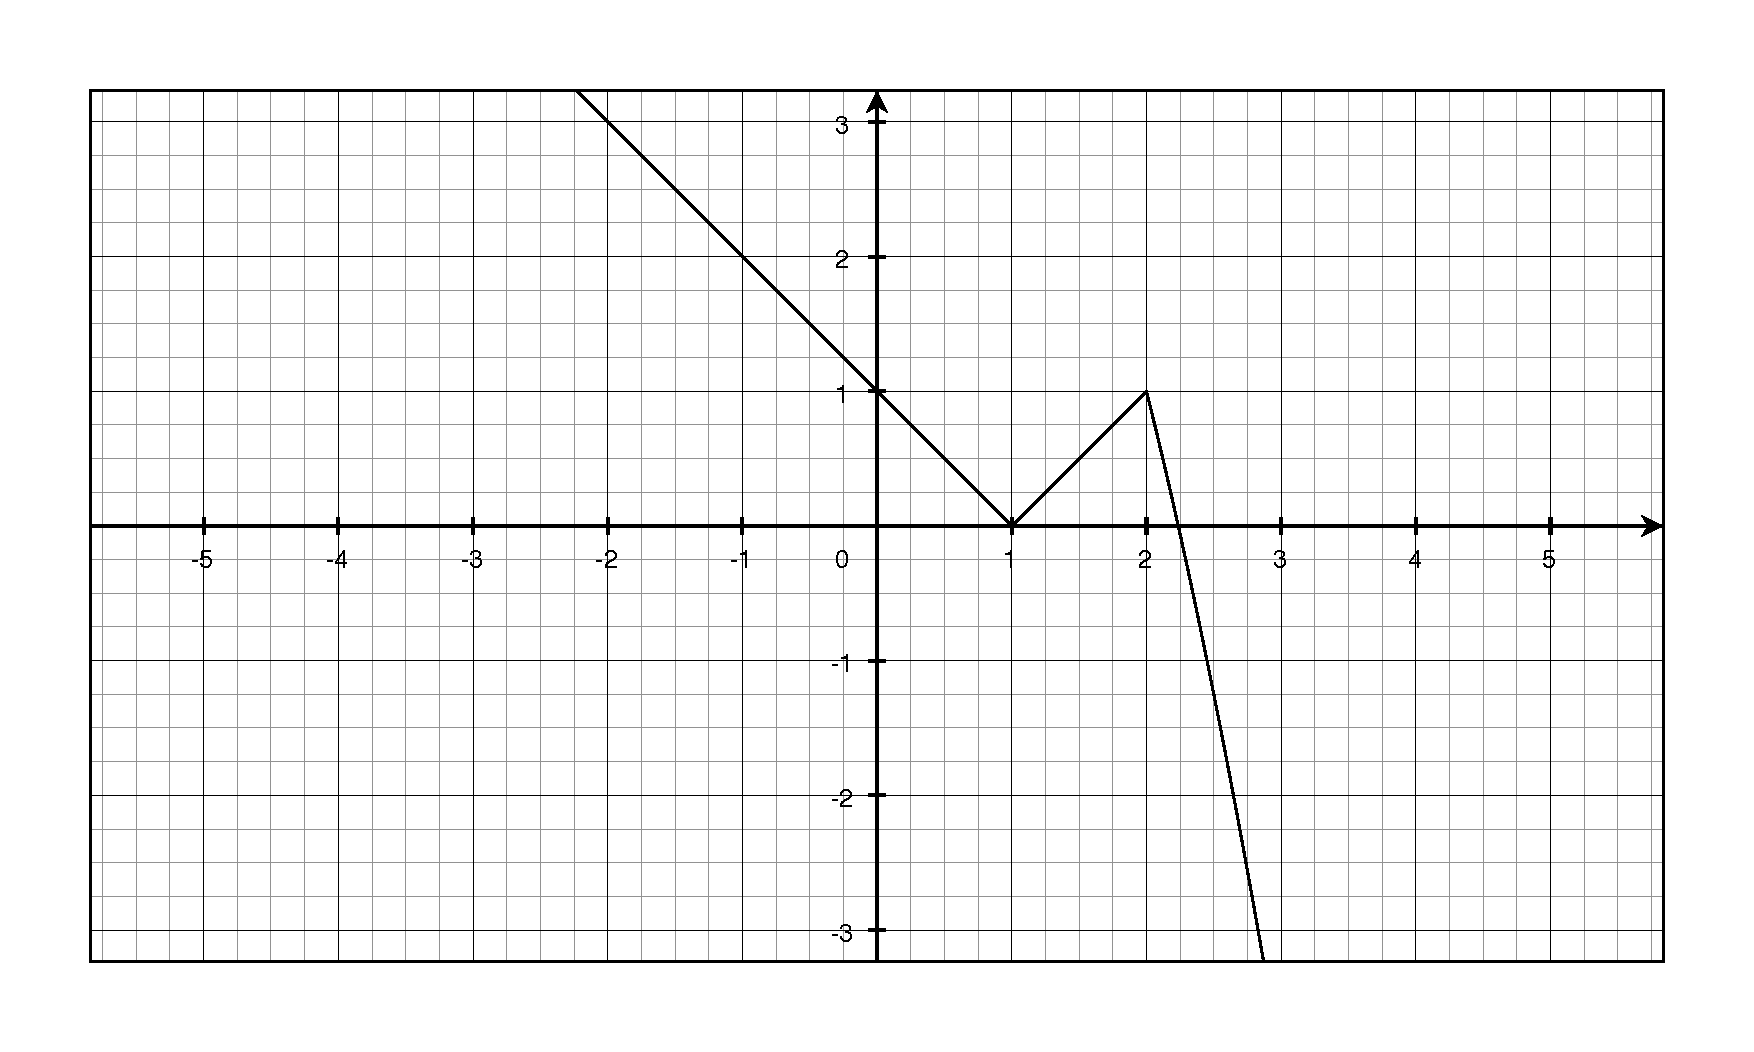
\includegraphics[scale=.3]{problem_30.eps}
      \caption*{Problem 30}
    \end{figure}

    \begin{enumerate}[(a)]

    \item $\lim_{x \to 1} g(x) = 0$
    \item $g(1)$ is not defined

    \item $\lim_{x \to 2} g(x) = 1$
    \item $\lim_{x \to 2^-} g(x) = 1$

    \end{enumerate}

  \end{description}

  \section{Section 2.5}
  \begin{description}

  \item[2]

  For any $\epsilon$ there is a $\delta$ such that if $|u - b| < \delta$ then $|g(u) - L| < \epsilon$.

  \item[7]
  To prove: for any $\epsilon$ there is a $\delta$ such that if $|x| < \delta$ then $|2x - 1 + 1| < \epsilon$.

  Preliminary Investigation:
  \begin{align*}
    |2x - 1 + 1| &< \epsilon \\
    2|x| &< \epsilon \\
    |x| &< \frac{\epsilon}{2} \\
  \end{align*}

  Select $\delta = \frac{\epsilon}{2}$ and show that if $|x| < \delta$ then $|2x - 1 + 1| < \epsilon$

  \begin{itemize}
    \item $|2x - 1 + 1| = 2|x|$
    \item $2|x| < 2 \delta$ since $|x| < \delta$
    \item $2 \delta = 2 \left( \frac{\epsilon}{2} \right) = \epsilon$
  \end{itemize}

  Putting it all together:
  \begin{align*}
    |2x - 1 + 1| = 2|x| &< 2 \delta = 2 \left( \frac{\epsilon}{2} \right) = \epsilon \\
    |2x - 1 + 1| < \epsilon \\
  \end{align*}

  Therefore, if $|x| < \delta$ then $|2x - 1 + 1| < \epsilon$ when $\delta = \frac{\epsilon}{2}$.

  \item[8]
  To prove: for any $\epsilon$ there is a $\delta$ such that 
  \[
    \text{ if } |x + 21| < \delta \text{ then } |3x - 1 + 64| < \epsilon.
  \]

  Preliminary Investigation:
  \begin{align*}
    |3x - 1 + 64| &< \epsilon \\
    3|x + 21| &< \epsilon \\
    |x + 21| &< \frac{\epsilon}{3} \\
  \end{align*}

  Select $\delta = \frac{\epsilon}{3}$ and show that if $|x + 21| < \delta$ then $|3x - 1 + 64| < \epsilon$

  \begin{itemize}
    \item $|3x - 1 + 64| = 3|x + 21|$
    \item $3|x + 21| < 3 \delta$ since $|x + 21| < \delta$
    \item $3 \delta = 3 \left( \frac{\epsilon}{3} \right) = \epsilon$
  \end{itemize}

  Putting it all together:
  \begin{align*}
    |3x - 1 + 64| = 3|x + 21| &< 3 \delta = 3 \left( \frac{\epsilon}{3} \right) = \epsilon \\
    |3x - 1 + 64| &< \epsilon
  \end{align*}

  Therefore, if $|x| < \delta$ then $|3x - 1 + 64| < \epsilon$ when $\delta = \frac{\epsilon}{3}$

  \item[9]
  To prove: For any $\epsilon$ there is a $\delta$ such that 
  \[
    \text{if } |x - 5| < \delta \text{ then } \left|\frac{x^2 - 25}{x-5} - 10\right| < \epsilon
  \]

  Preliminary Investigation:
  \begin{align*}
    \left| \frac{x^2 - 25}{x-5} - 10 \right| &< \epsilon \\
    \left| \frac{(x+5)(x-5)}{x-5} - 10 \right| &< \epsilon \\
    |x - 5| &< \epsilon \\
  \end{align*}

  Select $\delta = \epsilon$ and show that if $|x - 5| < \delta$ then $\left| \frac{x^2 - 25}{x-5} - 10 \right| < \epsilon$

  \begin{itemize}
    \item $\left| \frac{x^2 - 25}{x-5} - 10 \right| = \left| x - 5 \right|$
    \item $\left| x - 5 \right| < \delta$
    \item $\delta = \epsilon$
  \end{itemize}

  Putting it all together:
  \begin{align*}
    \left| \frac{x^2 - 25}{x-5} - 10 \right| = | x - 5 | &< \delta = \epsilon \\ 
    \left| \frac{x^2 - 25}{x-5} - 10 \right| &< \epsilon \\ 
  \end{align*}

  Therefore, if $|x - 5| < \delta$ then $\left| \frac{x^2 - 25}{x-5} - 10 \right| < \epsilon$ when $\delta = \epsilon$.

  \pagebreak

  \item[10]
  To prove: For any $\epsilon$ there is a $\delta$ such that 
  \[
    \text{if } |x| < \delta \text{ then } \left|\frac{2x^2 - x}{x} + 1\right| < \epsilon
  \]

  Preliminary Investigation:
  \begin{align*}
    \left|\frac{2x^2 - x}{x} + 1\right| &< \epsilon \\
    |2x - 1 + 1| &< \epsilon \\
    |2x| &< \epsilon \\
    |x| &< \frac{\epsilon}{2} \\
  \end{align*}

  Select $\delta = \frac{\epsilon}{2}$ and show that if $|x| < \delta$ then $\left|\frac{2x^2 - x}{x} + 1\right| < \epsilon$

  \begin{itemize}
    \item $\left|\frac{2x^2 - x}{x} + 1\right| = |2x| = 2|x|$
    \item $2|x| < 2 \delta$ since $|x| < \delta$.
    \item $2 \delta = 2 \left( \frac{\epsilon}{2} \right) = \epsilon$
  \end{itemize}

  Putting it all together:
  \begin{align*}
    \left|\frac{2x^2 - x}{x} + 1\right| = 2|x| &< 2 \delta = 2 \left( \frac{\epsilon}{2} \right) = \epsilon \\ 
    \left|\frac{2x^2 - x}{x} + 1\right| &< \epsilon \\ 
  \end{align*}

  Therefore, if $|x| < \delta$ then $\left|\frac{2x^2 - x}{x} + 1\right| < \epsilon$ when $\delta = \frac{\epsilon}{2}$.

  \pagebreak

  \item[11]
  To prove: For any $\epsilon$ there is a $\delta$ such that 
  \[
    \text{if } |x - 5| < \delta \text{ then } \left|\frac{2x^2 - 11x + 5}{x-5} -9 \right| < \epsilon
  \]

  Preliminary Investigation:
  \begin{align*}
    \left|\frac{2x^2 - 11x + 5}{x-5} -9 \right| < \epsilon \\
    \left|\frac{(2x - 1)(x-5)}{x-5} -9 \right| < \epsilon \\
    |2x - 1 - 9| &< \epsilon \\
    |2x - 10| &< \epsilon \\
    2|x - 5| &< \epsilon \\
    |x - 5| &< \frac{\epsilon}{2} \\
  \end{align*}

  Select $\delta = \frac{\epsilon}{2}$ and show that if $|x - 5| < \delta$ then 
  \[
    \left|\frac{2x^2 - 11x + 5}{x-5} -9 \right| < \epsilon
  \]

  \vspace{0.2 cm}

  \begin{itemize}
    \item $\left|\frac{2x^2 - 11x + 5}{x-5} -9 \right| = 2|x-5|$
    \item $2|x - 5| < 2 \delta$ since $|x - 5| < \delta$.
    \item $2 \delta = 2 \left( \frac{\epsilon}{2} \right) = \epsilon$
  \end{itemize}

  Putting it all together:
  \begin{align*}
    \left|\frac{2x^2 - 11x + 5}{x-5} -9 \right| = 2|x-5| &< 2 \delta = 2 \left( \frac{\epsilon}{2} \right) = \epsilon \\ 
    \left|\frac{2x^2 - 11x + 5}{x-5} -9 \right| &< \epsilon \\ 
  \end{align*}

  Therefore, if $|x - 5| < \delta$ then $\left|\frac{2x^2 - 11x + 5}{x-5} -9 \right| < \epsilon$ when $\delta = \frac{\epsilon}{2}$.

  \item[12]
  To prove: For any $\epsilon$ there is a $\delta$ such that 
  \[
    \text{if } |x - 1| < \delta \text{ then } | \sqrt{2x} - \sqrt{2} | < \epsilon
  \]

  Preliminary Investigation:
  \begin{align*}
    | \sqrt{2x} - \sqrt{2}| < \epsilon \\
    \left| \sqrt{2x} - \sqrt{2} \left( \frac{\sqrt{2x} + \sqrt{2}}{\sqrt{2x} + \sqrt{2}} \right) \right| < \epsilon \\
    \left| \frac{2x - 2}{\sqrt{2x} + \sqrt{2}} \right| < \epsilon \\
    \left| \frac{2(x - 1)}{\sqrt{2}(x + 1)} \right| < \epsilon \\
    \sqrt{2} \left| \frac{x - 1}{\sqrt{x} + 1} \right| < \epsilon \\
    \\
    \left| \frac{x - 1}{\sqrt{x} + 1} \right| \leq |x - 1| \text{ since } \sqrt{x} \geq 0 \\
    \\
    \sqrt{2} | x - 1| < \epsilon \\
    | x - 1| < \frac{\epsilon}{\sqrt{2}} \\
  \end{align*}

  Select $\delta = \frac{\epsilon}{\sqrt{2}}$ and show that if $|x - 1| < \delta$ then $\left|\sqrt{2x} - \sqrt{2} \right| < \epsilon$

  \vspace{0.2 cm}

  \begin{align*}
    | \sqrt{2x} - \sqrt{2}| = \sqrt{2} \left| \frac{x - 1}{\sqrt{x} + 1} \right| &\leq  \sqrt{2} | x - 1| \\
        &< \sqrt{2} \cdot \delta = \sqrt{2} \left( \frac{\epsilon}{\sqrt{2}} \right) = \epsilon \\ 
    | \sqrt{2x} - \sqrt{2}| &< \epsilon \\ 
  \end{align*}

  Therefore, if $|x - 1| < \delta$ then $| \sqrt{2x} - \sqrt{2}| < \epsilon$ when $\delta = \frac{\epsilon}{\sqrt{2}}$.

  \end{description}
  \else

  \vspace{10 cm}

  {\em I can't understand why people are frightened of new ideas. I'm frightened of the old ones.}

  \vspace{.2 cm}

  \hspace{1 cm} --John Cage

  \fi

\end{document}

